%%=============================================================================
%% Results
%%=============================================================================

\chapter{\IfLanguageName{dutch}{Resultaten}{Results}}%
\label{ch:results}

The result section focuses on elaborating conducted experiments and acquired results, divided into the three main phases, localization, segmentation and recognition. In order to label, annotate videos and gain insights in the results a Vue3 web-app is created on a python flask API which reads and stores labels and video annotations from a MySQL database. Furthermore, the experiments are all performed using an Acer Nitro ANV15-51, running Ubuntu 24.04.2 LTS, using a 13th Gen Intel® Core™ i5-13420H × 12, with 16GB RAM and a NVIDIA GeForce RTX™ 4050 Laptop GPU (6GB).

\section{Jumper localization}

% TODO: add, this is relevant
% TODO: convex hull the 3 jumpers and train on yolo model.
As DD3 routines are the focus of this research, the idea was to predict the coordinates and position of a team as a single unit, instead of individuals. This idea was supported by the fact that there aren't any public jump rope datasets and it was expected to increase the speed of labeling. The AI generated image \ref{fig:sr2-performance-ai-generated} shows an example of a competition setting where two athletes are performing a routine. The goal here would be to crop out the jumpers.

Below you can find a shortlist of experiments executed on localization.

\begin{itemize}
    \item random conv
    \item googlenet, mobilenet...
    \item Mask-RCNN
    \item Labeling individual jumpers \& pre-trained model yolo -> OK
\end{itemize}

\subsection{Random convolutional network}

% TODO : illustrative image of box coords?

Before discussing the different results, let's discuss how the location of skippers are marked. To mark the position of an object on an image, there are multiple possibilities.
For this project, the relative center point along the x-axis, y-axis, width and height of the box are stored. So regardless of the scale of the image, whether the image has size 1920 x 1080 pixels or 1080 x 720 pixels, the position of the box remains the same.
An example of a box would be [0.6, 0.5, 0.4, 0.4], all values between 0 and 1. IoU accuracy can then be performed.
... As explained in the literature (todo reference to lit)...
% TODO : shift IoU comparison to literature

In order to get an idea, whether following models are able to learn, a random convolutional network is created.
... elaborate results % TODO

-> low accuracy, naive predictions.

To get a first idea whether it would start learning, so a transition can be made towards more advanced architectures.

\subsection{Dedicated architectures}

From scratch

GoogleNet, MobileNet... (on individual labels)

Conclusion:
Predicting full teams didn't work out which allowed for a transition to labeling and predicting individuals athletes. Below you find more information about those experiments.

\subsection{Mask-RCNN}
Failed experiment, C error, no results.

\subsection{YOLO}

Experiment 3, pre-trained models \& individual boxes.

The third experiment incorporates a double upgrade. The first upgrade involves annotating individual athletes on images instead of one big box around all jumpers, which allows more varying labels on collected single rope or double dutch 4 videos. The second upgrade is trying a pre-trained object detection model.

Ultralytics \autocite{Khanam2024} provides an easy-to-use pre-trained implementation for predicting people and objects in images which can be fine-tuned for specific use cases. Fine-tuning was needed as spectators, also humans, were also included in the predictions.

Using these predictions, a crop around the three jumpers can be created using the predicted jumper boxes from the fine-tuned YOLO model, after using the pre-trained weights on the COCO dataset \autocite{Lin2014}. In order to improve the crops some steps were required. Details are discussed below.

\subsubsection{Eliminate spectators - IoU comparison}

\begin{figure}
    \centering
    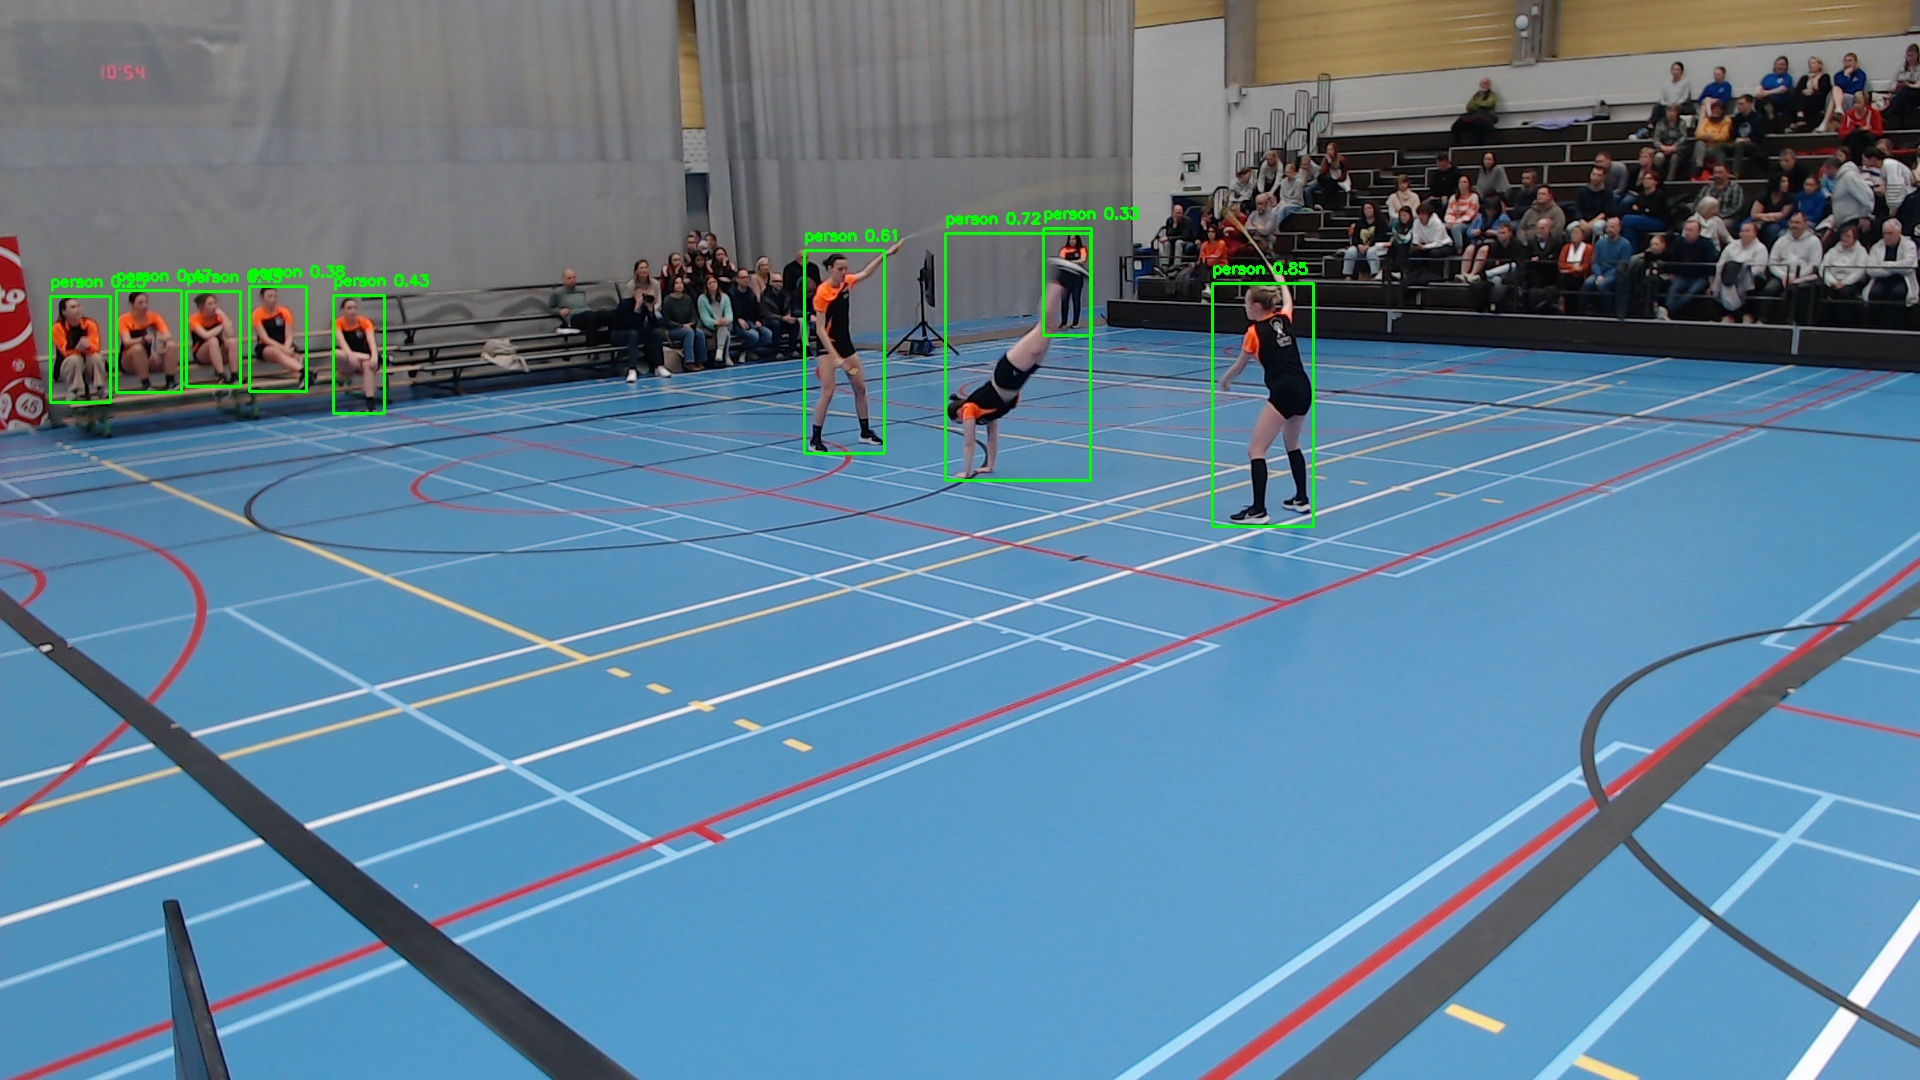
\includegraphics[width=0.95\linewidth]{img/1267_292_boxes}
    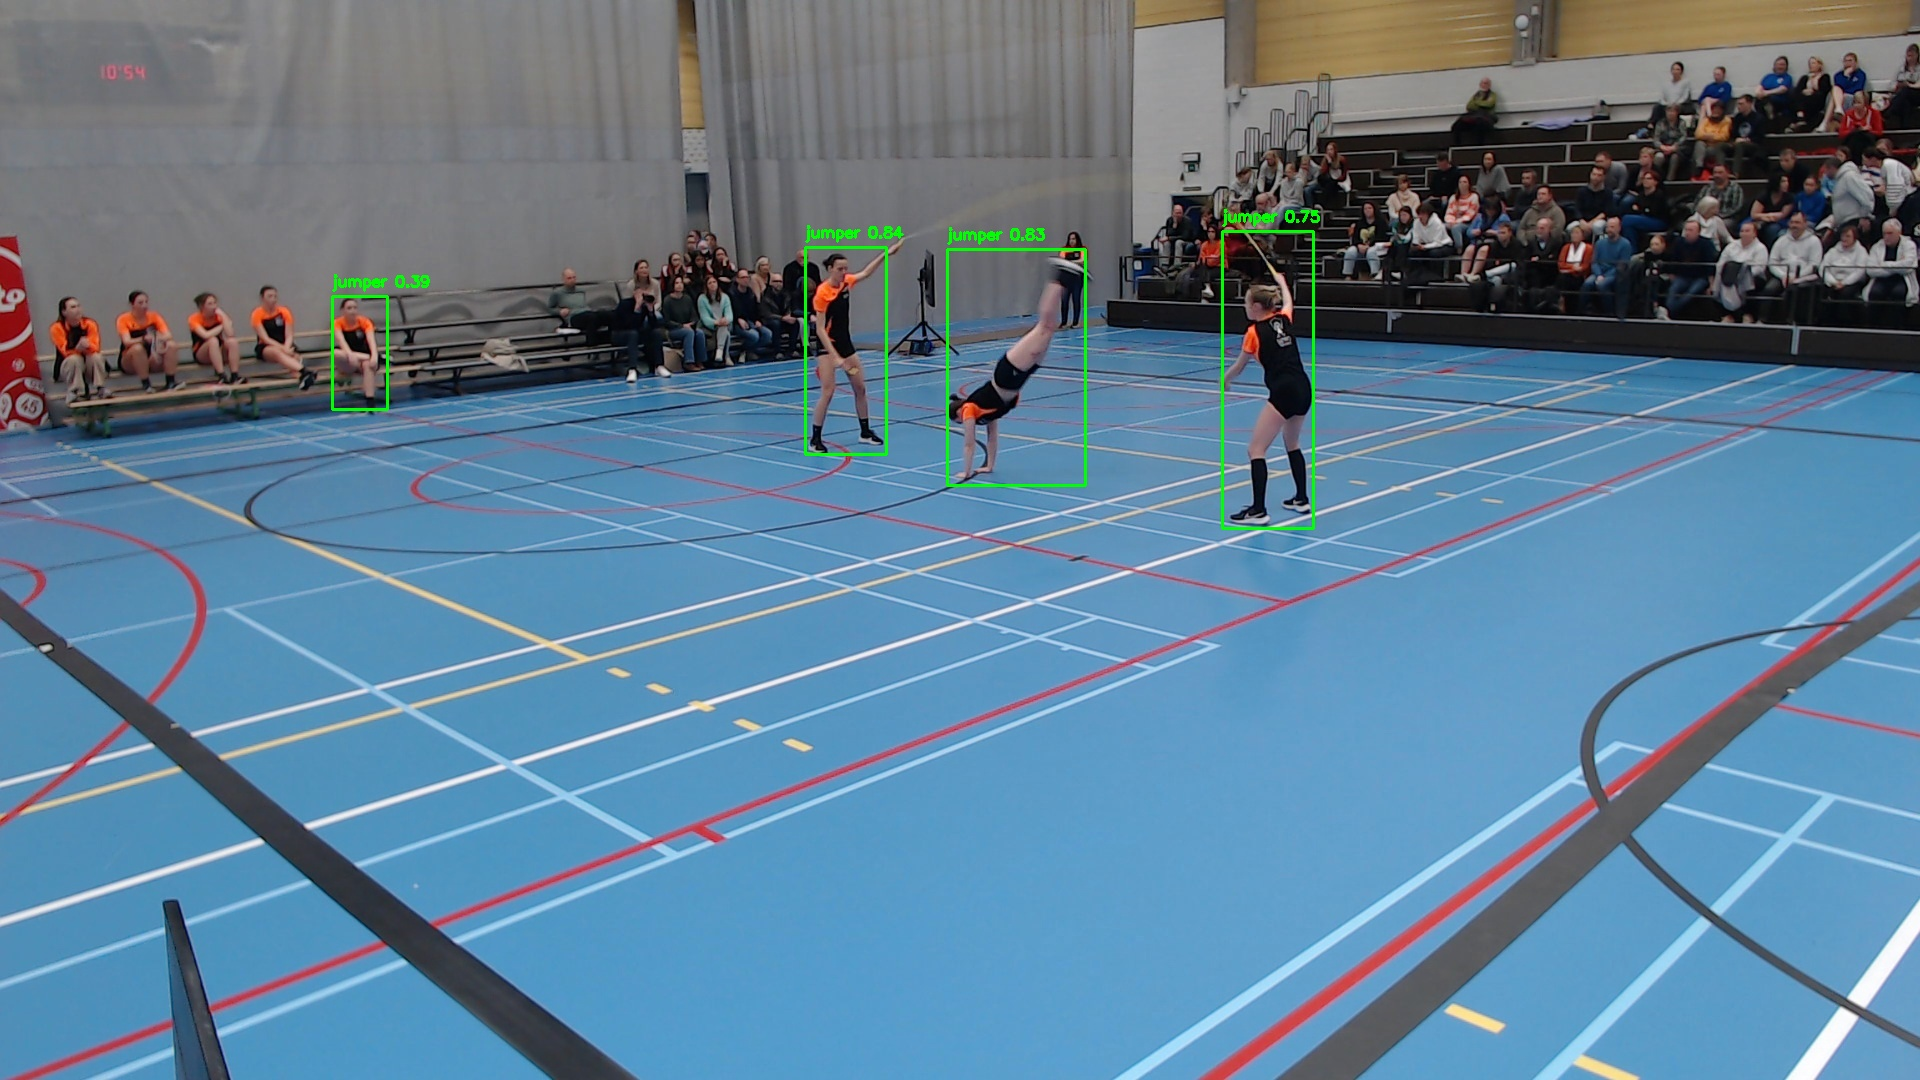
\includegraphics[width=0.95\linewidth]{img/1267_292_boxes_reduced_spectators}
    \caption[raw vs fine-tuned YOLOv11 nano model predictions]{Raw predictions of the unrefined YOLOv11 nano model compared to the fine-tuned model which reduces predictions of spectators.}
    \label{fig:raw-vs-fine-tuned-boxes}
\end{figure}

\begin{figure}
    \centering
%%    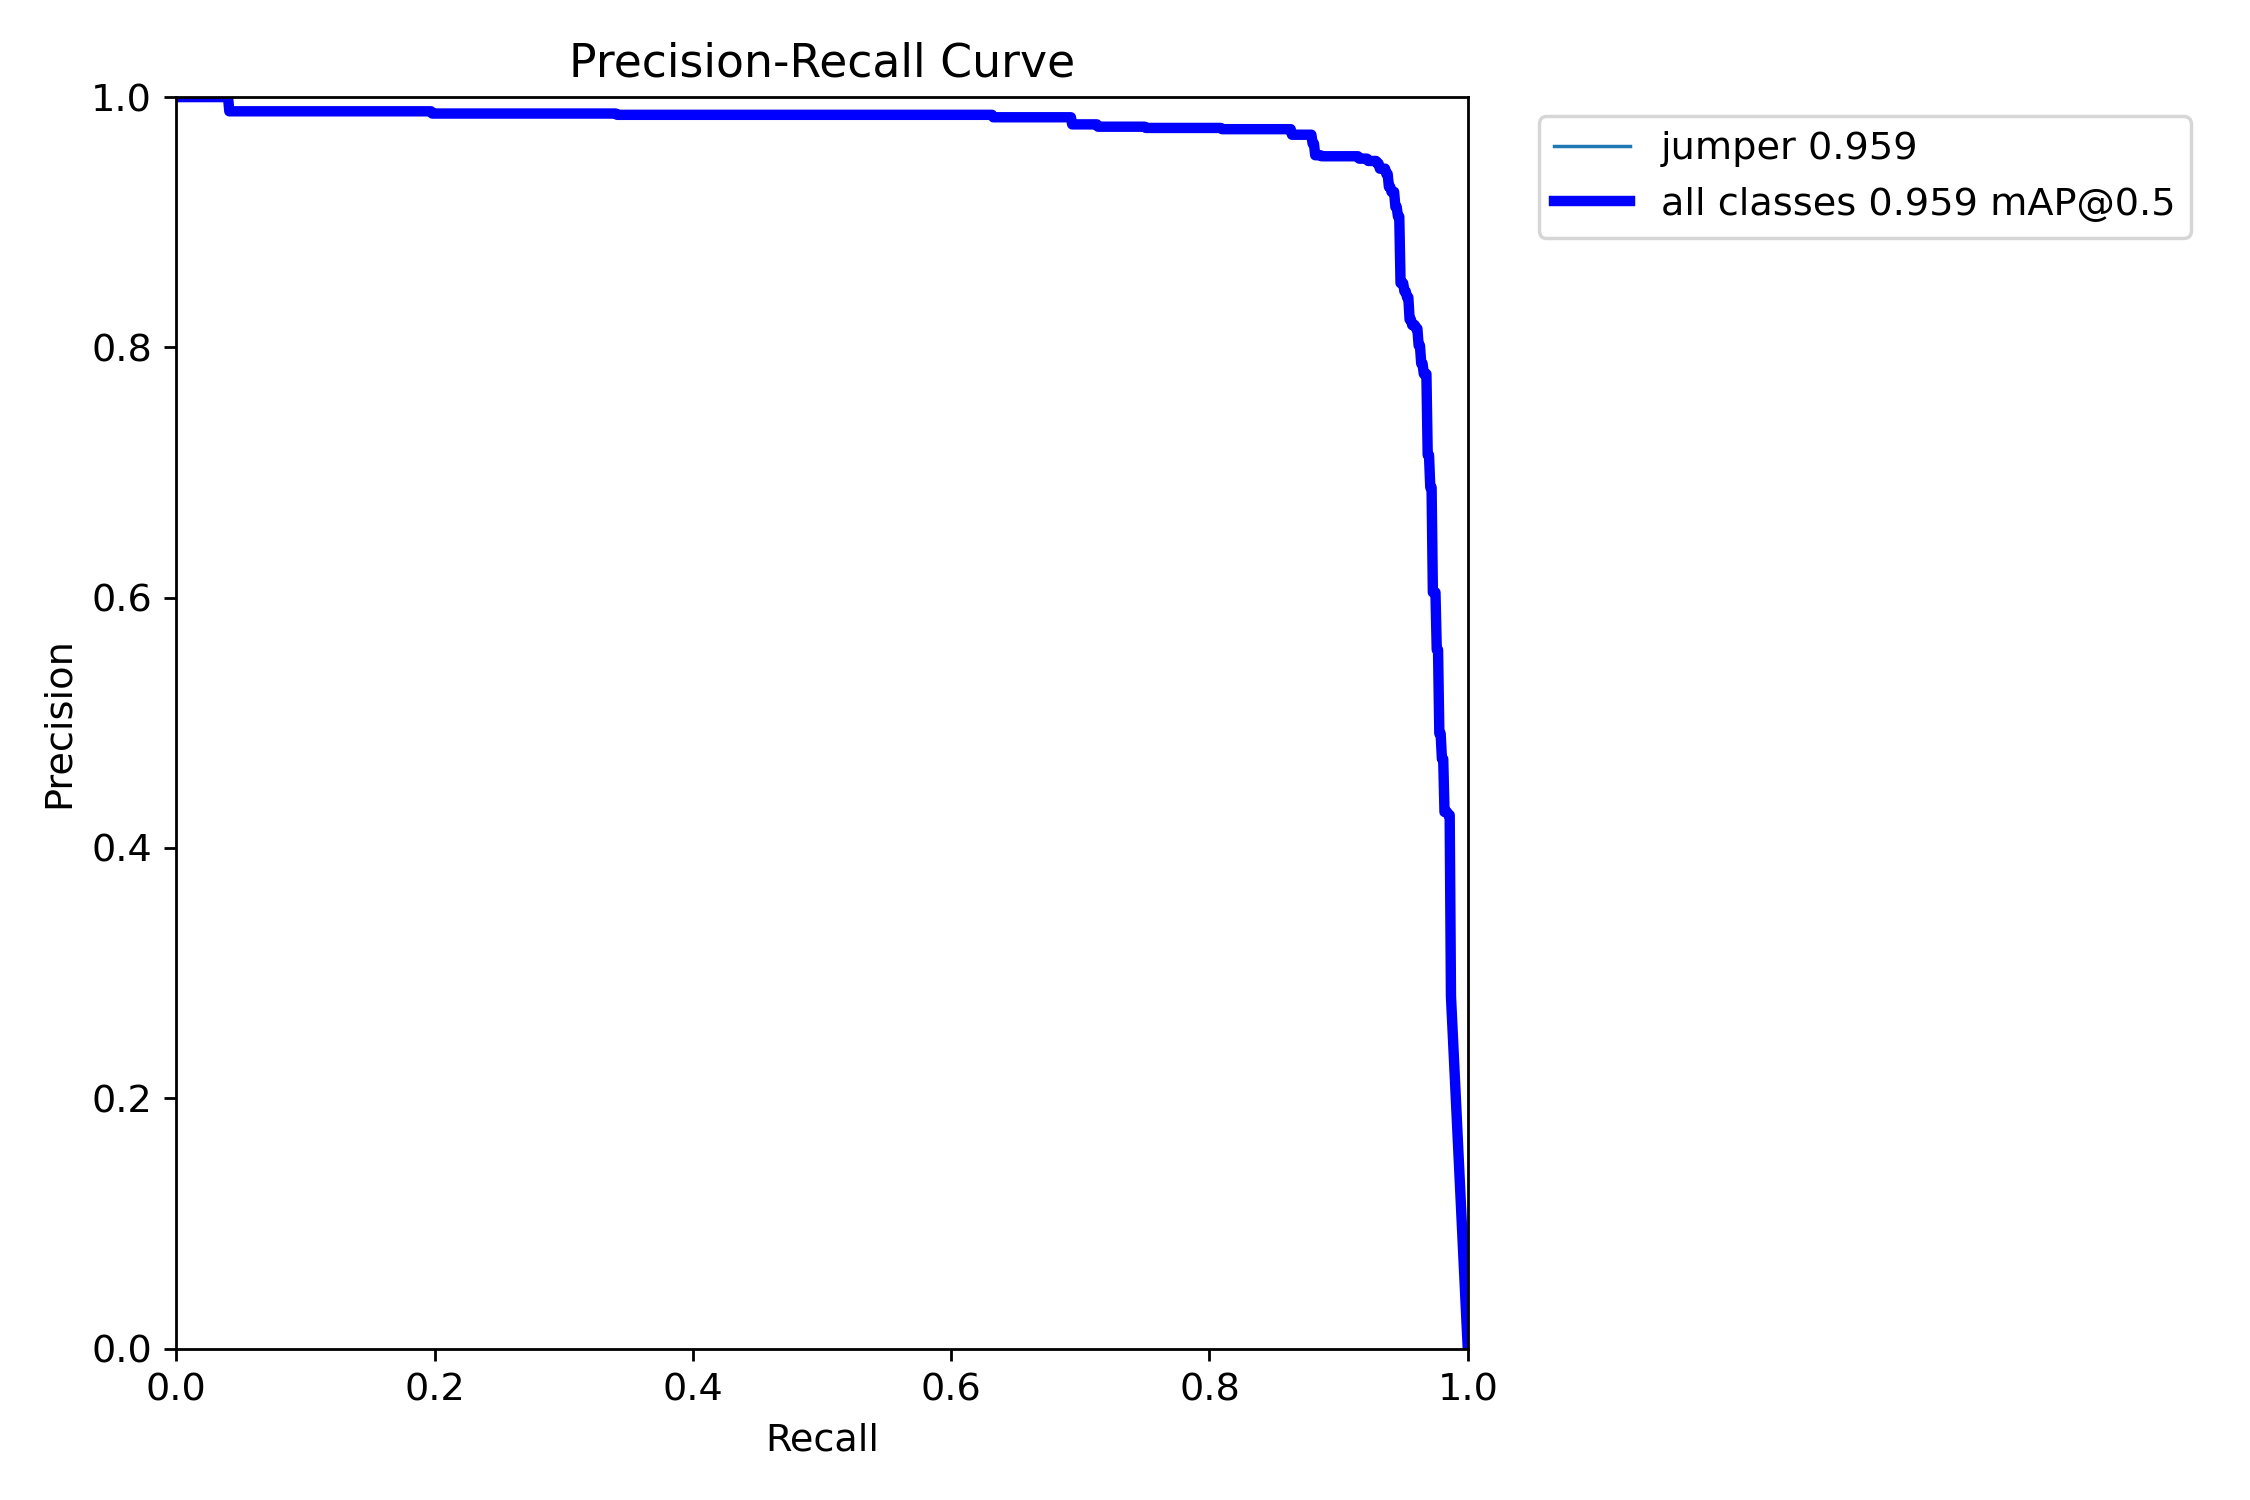
\includegraphics[width=0.35\linewidth]{img/PR_curve}
    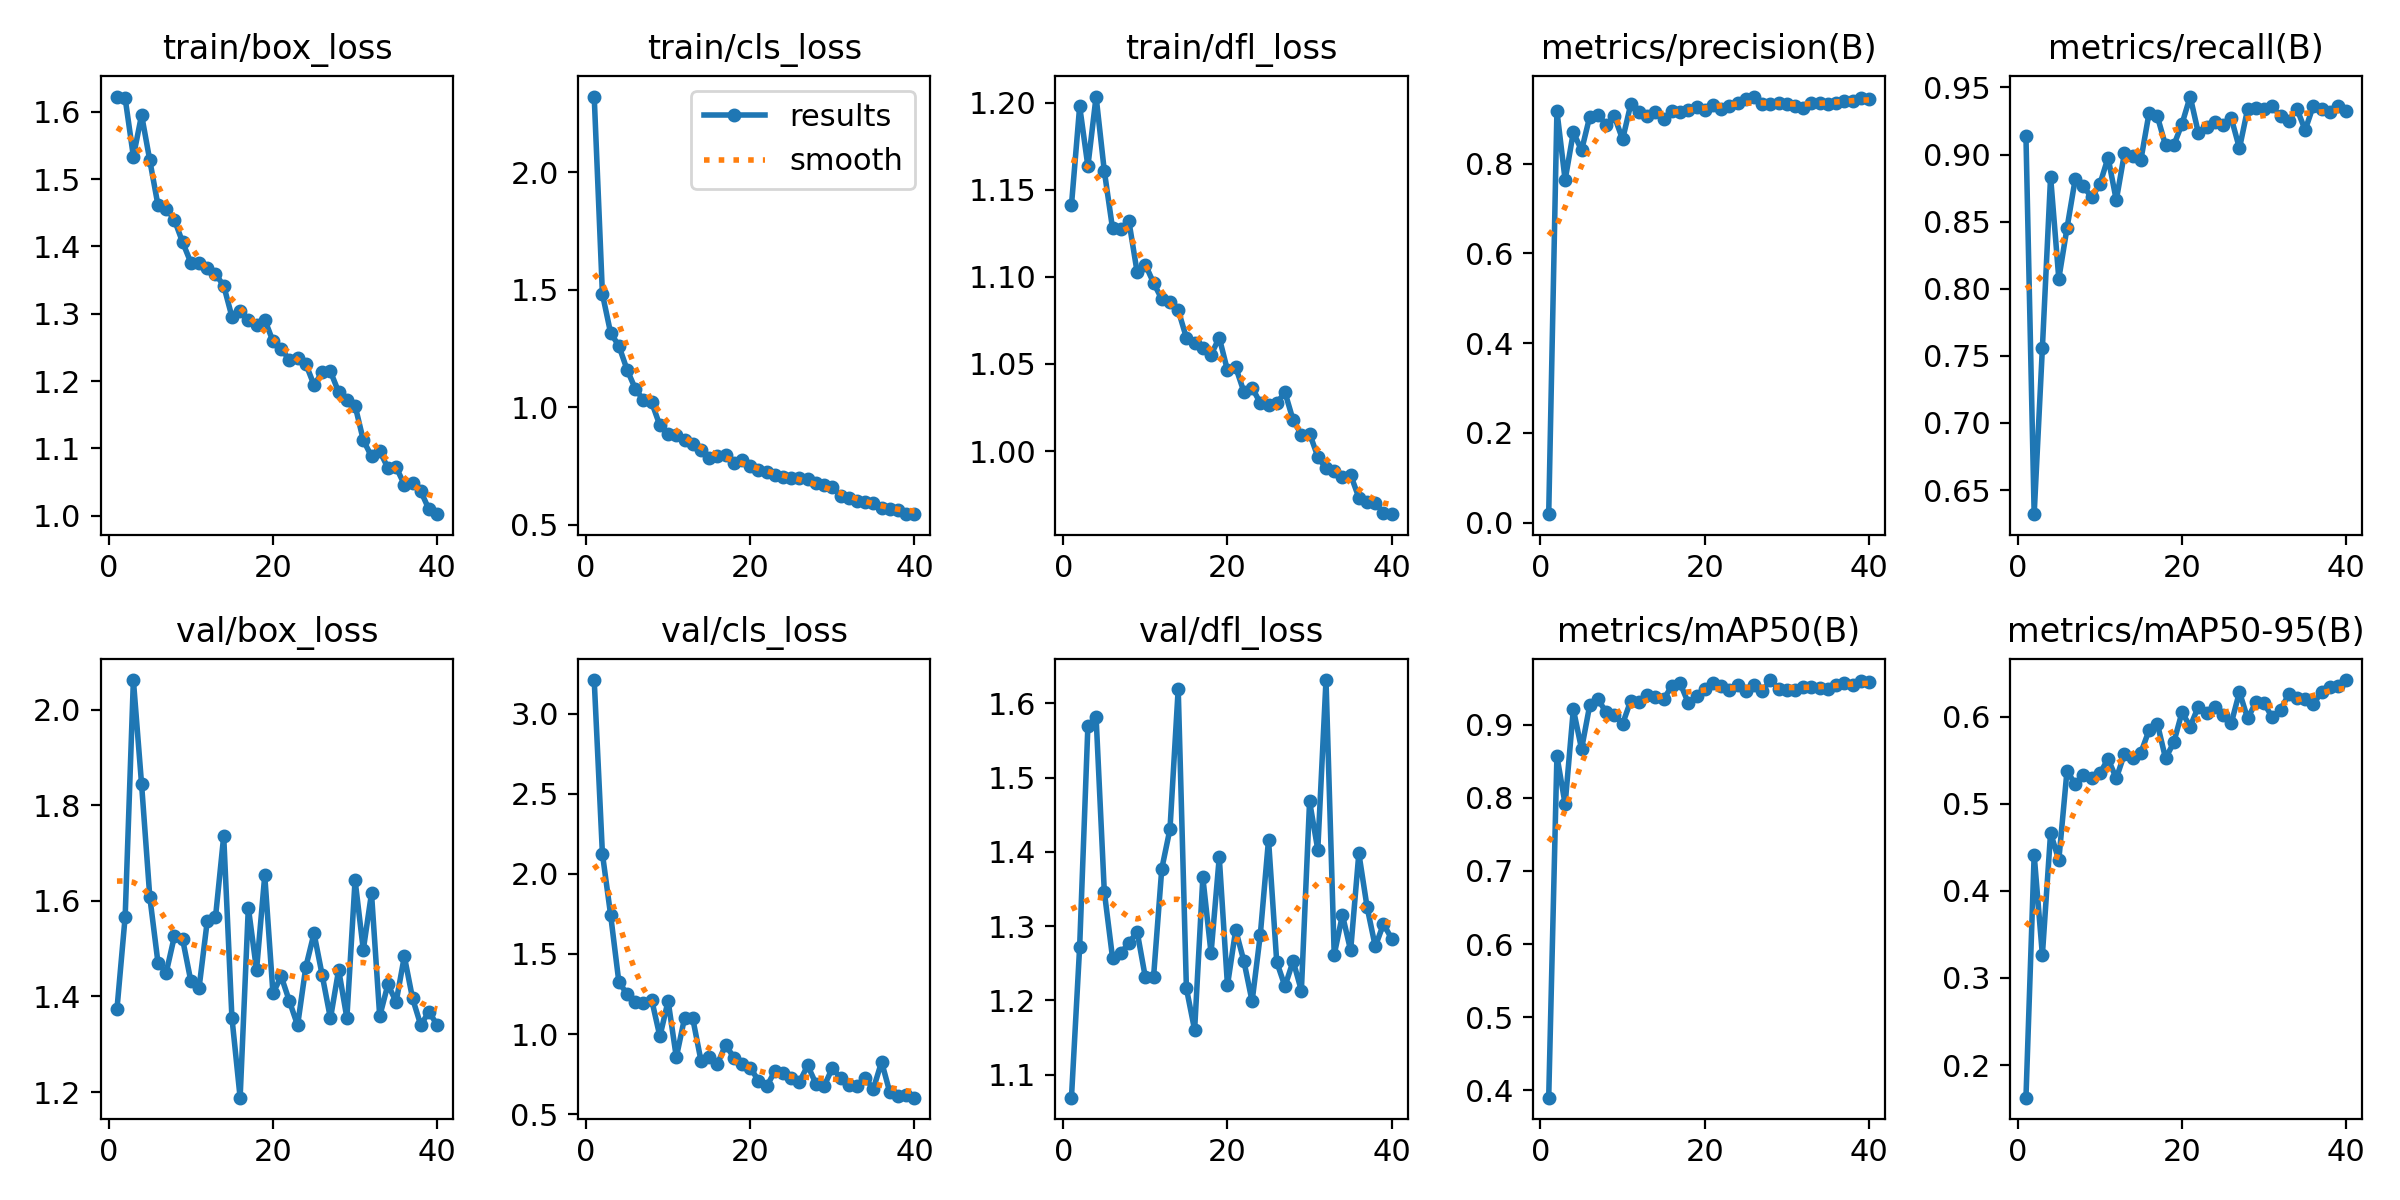
\includegraphics[width=0.95\linewidth]{img/results}
    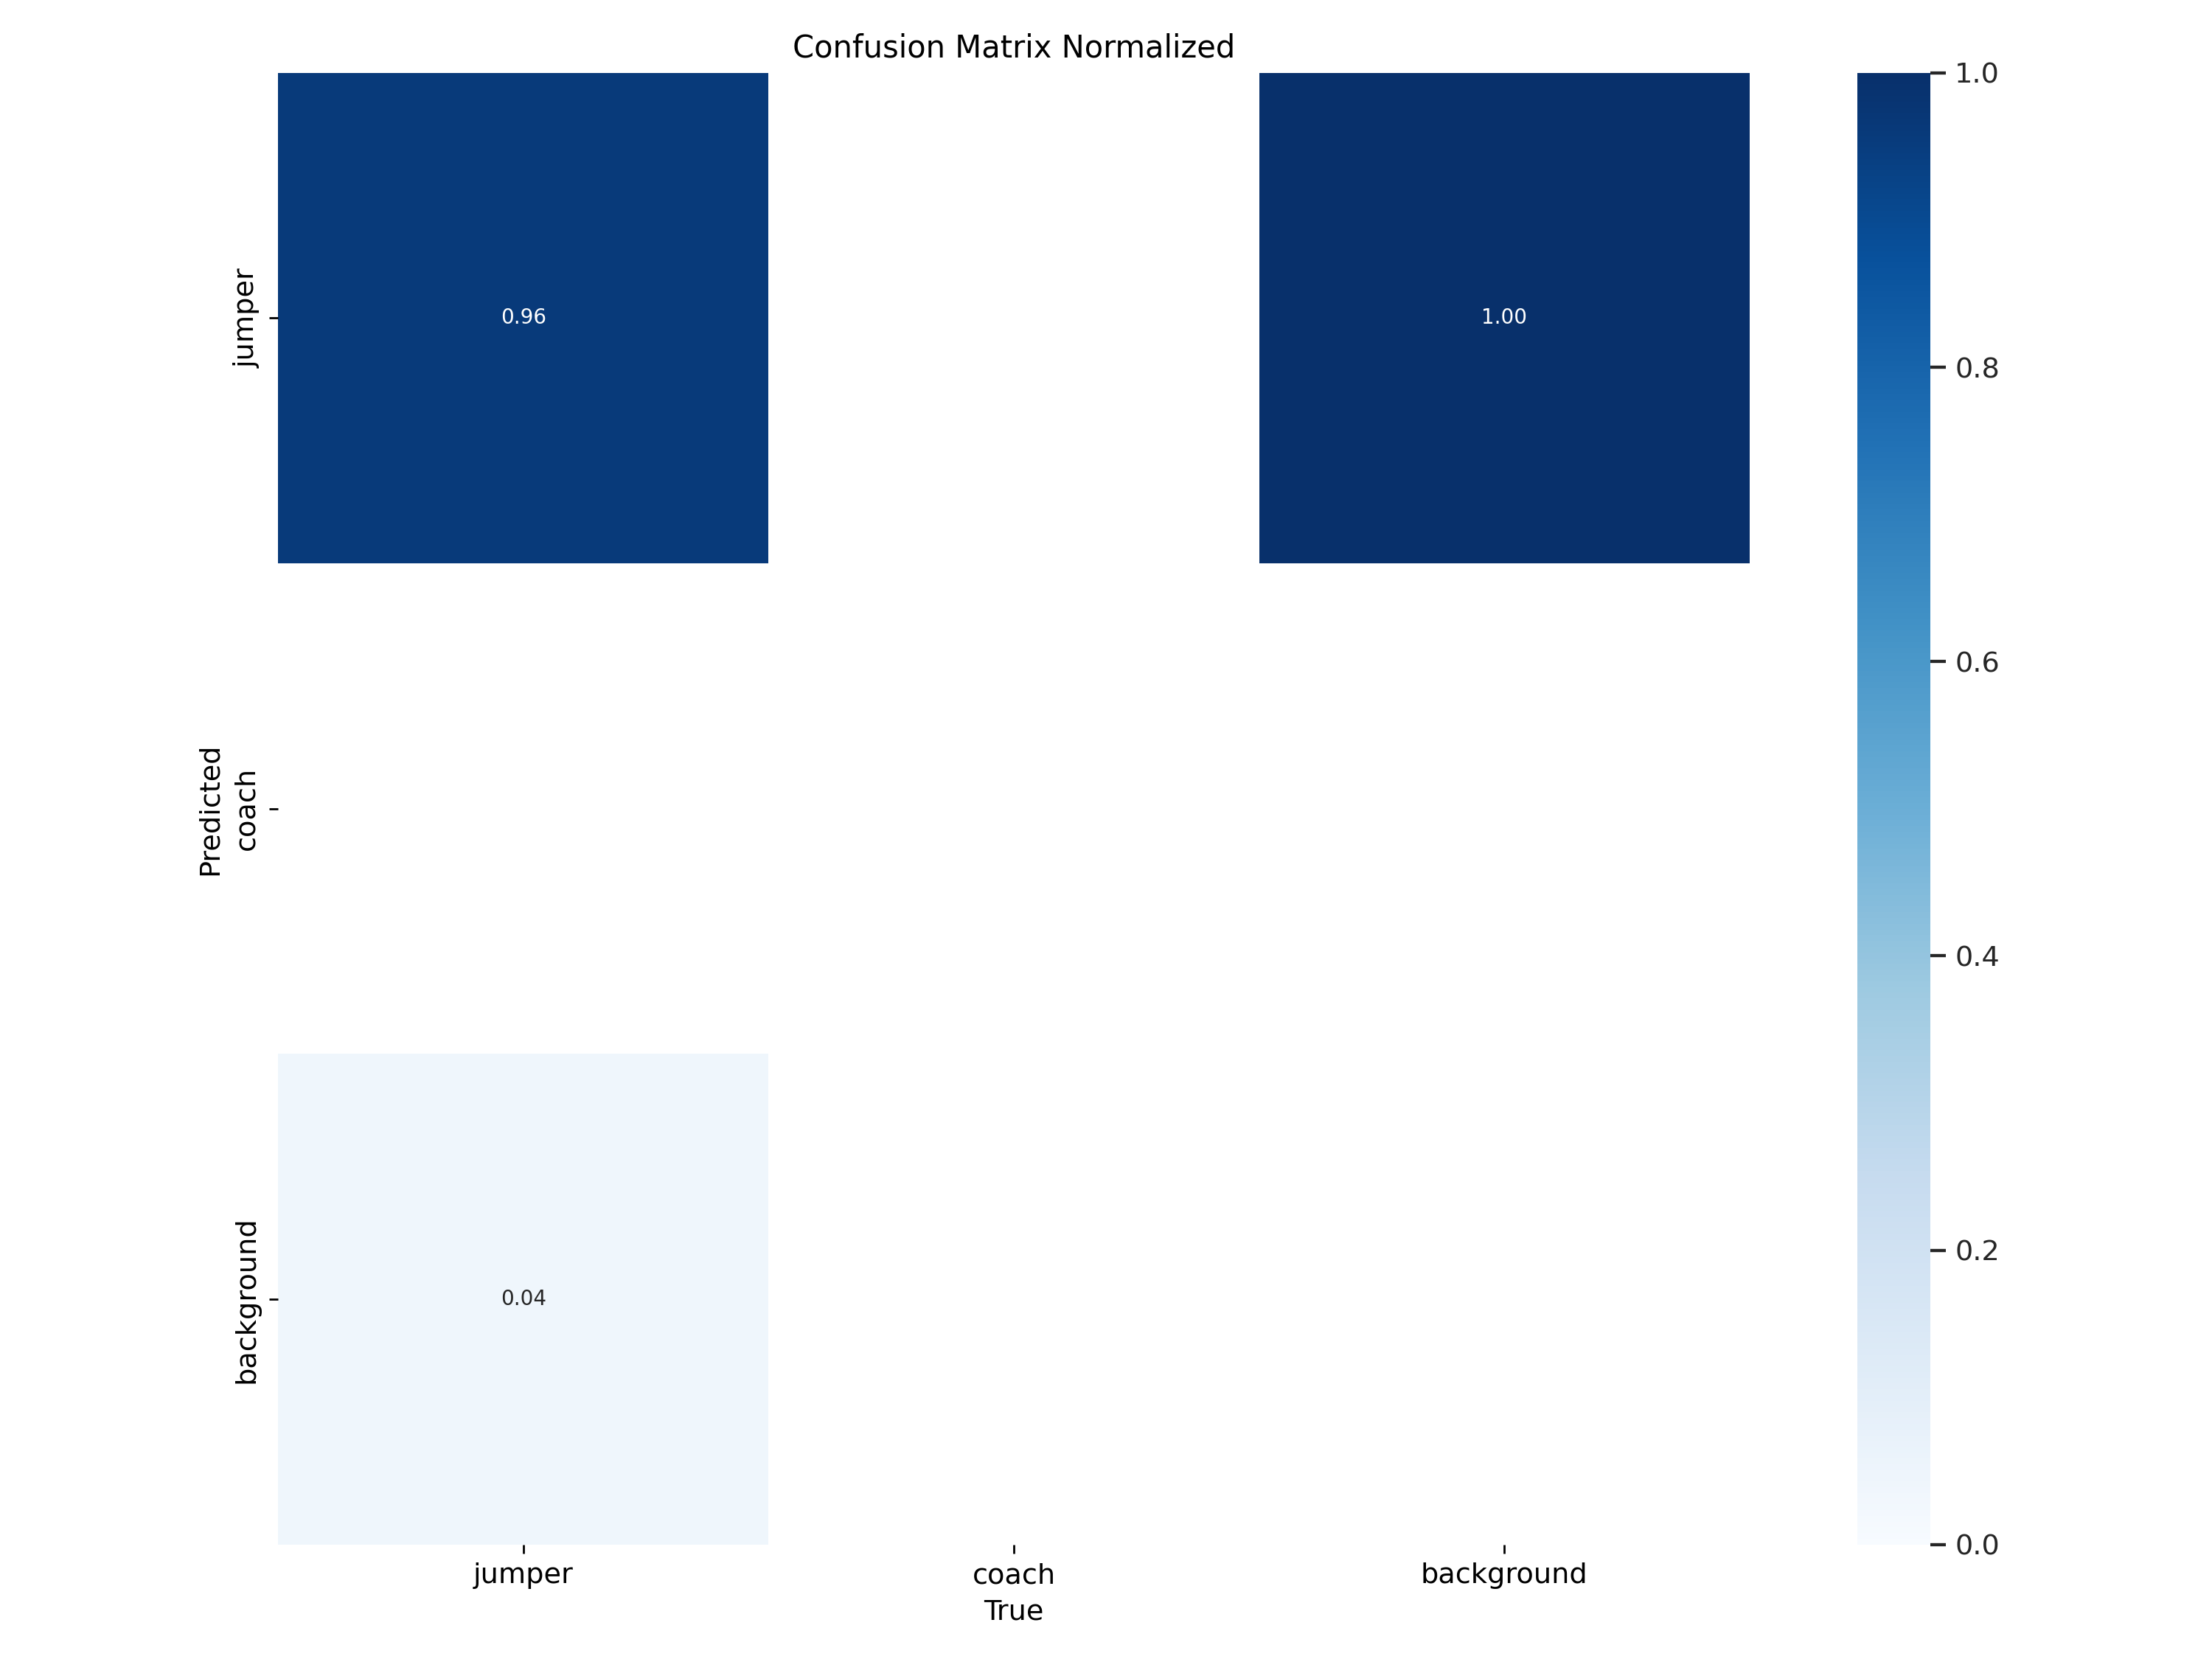
\includegraphics[width=0.85\linewidth]{img/confusion_matrix_normalized}
    \caption[metrics after fine-tuning YOLOv11]{Metrics after fine-tuning YOLOv11 on the validation set of 161 images}
    \label{fig:localization-results}
\end{figure}

In order to eliminate the spectators, coaches or judges, only athletes are marked on images. Using 729 annotated frames as refinement, predictions of spectators are reduced considerately, while occasional spectators are still predicted. See figure \ref{fig:raw-vs-fine-tuned-boxes} for clarity.
This results in imperfect crops \ref{fig:dd3-crop-error} as compared to valid crops \ref{fig:dd3-crop}.

See

In order to reach stability in the predictions, box-coordinates of the last
Even though the model is fine-tuned on almost two-thousand images, occasionally coaches or spectators were still predicted as jumpers, requiring a solution.
When a spectator or more than one is predicted, this means that total crop of all 'athletes' could be bigger than the actual location of all jumpers. A comparison in overlap between previous predictions (N seconds) and the current prediction enables the possibility to keep the crop position of the previous frame for the current frame. Comparing overlap is called Intersection over Union or IoU for short.

(Clarifying images will follow in a next version)

A possible improvement could be matching previous boxes with the new predictions, eliminating the spectator. Which begs the question, what if the jumpers are entering the field? There are no earlier predicted boxes to match.

\begin{figure}
    \centering
    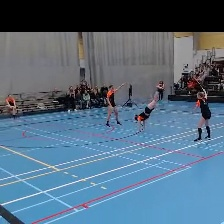
\includegraphics[width=0.45\linewidth]{img/1267_292_cropped}
    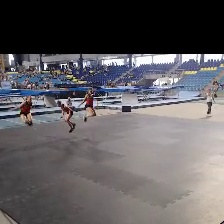
\includegraphics[width=0.45\linewidth]{img/1405_1061_cropped}
    \caption[dd3-crop-error]{Two crops were a spectator alongside the athletes.}
    \label{fig:dd3-crop-error}
\end{figure}

\begin{figure}
    \centering
    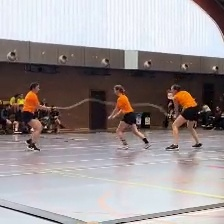
\includegraphics[width=0.45\linewidth]{img/1315_2935}
    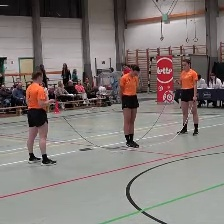
\includegraphics[width=0.45\linewidth]{img/2297_134}
    \label{fig:dd3-crop}
    \caption[Valid crops of a DD3 routine on competition.]{Valid crops of a DD3 routine on competition.}
\end{figure}

\subsection{Eliminate shakiness}

A video is a sequence of frames changing the position of the skipper a little bit each frame. Even if actions are fluidly executed, the actual predictions of the jumpers location can shift a few pixels to the left or right between consecutive boxes. This means that raw crops are shaking around the jumper, disturbing the natural feel.

Smoothing values (S), two parameters, where added to eliminate the shaking of consecutive crops. One of the parameters is used for smoothly shrinking the frame (0.94), the other for expanding the frame (0.85).
This means that the crop of a new frame is S times the crop value of the previous frame added with 1 - S times the new prediction, elimination shakiness. The second parameter was added in order to fix jumpers running out the crop while executing a larger actions covering a lot of position on the floor.

It was playing around with these parameters (smooth values \& N) to get a working setup which works in most cases, sporadically changing one if the crop of a video was not sufficient, e.g. running out of the cropped view.

Full code:

\begin{listing}
   \begin{minted}{python}
       print('TODO : cleanup code')
   \end{minted}
   \caption[Example codefragment]{Example of adding cropping code.}
\end{listing}


\section{Action segmentation}

\section{Skill recognition}

The first trials from scratch, a video vision transformer, which is adapted from the transformer created during classes. Adding the convolution layer in front and the time dimension created the ViViT transformer as proposed in (source).
Idea's add extra convolution layers \& use pre-trained model.

Elaborate 16 frame time aspect.

\subsection{Video Vision Transformer}

For training the video vision transformer, the data is upsampeled

\subsection{Multiscale Video Vision Transformer - MViT}
\href{https://pytorch.org/vision/main/models/video_mvit.html}{Pytorch MViT}

Pytorch implementation of source.

For the first training round a double upgrade has been performed. The first adaption is downsampling the skills in 5 main classes to predict.  \& pre-trained model.

\begin{table}[h!]
    \centering
    \begin{tabular}{|r|r|l|r|r|}
        \hline
        \textbf{Train \%} & \textbf{Train Count} & \textbf{Skill} & \textbf{Val Count} & \textbf{Val \%} \\
        \hline
        50.6687 & 2273 & jump & 379 & 56.6517 \\
        14.0660 & 631 & pushup & 77 & 11.5097 \\
        13.0629 & 586 & return from power & 84 & 12.5561 \\
        9.8529 & 442 & frog & 59 & 8.8191 \\
        3.2100 & 144 & crab & 9 & 1.3453 \\
        2.0062 & 90 & split & 12 & 1.7937 \\
        1.1146 & 50 & flip & 5 & 0.7474 \\
        0.9140 & 41 & rondat & 5 & 0.7474 \\
        0.8917 & 40 & rad & 3 & 0.4484 \\
        0.8025 & 36 & suicide & 8 & 1.1958 \\
        0.7356 & 33 & handspring & 5 & 0.7474 \\
        0.6910 & 31 & rol2kip & 7 & 1.0463 \\
        0.4458 & 20 & kip & 6 & 0.8969 \\
        0.3567 & 16 & speed & NULL & NULL \\
        0.3121 & 14 & kopkip & 1 & 0.1495 \\
        0.2675 & 12 & roll & 3 & 0.4484 \\
        0.1783 & 8 & stut & 2 & 0.2990 \\
        0.1337 & 6 & swift & NULL & NULL \\
        0.1337 & 6 & UNKOWN & 1 & 0.1495 \\
        0.0669 & 3 & leapfrog & NULL & NULL \\
        0.0446 & 2 & footwork-kick & NULL & NULL \\
        0.0223 & 1 & mountainclimber & NULL & NULL \\
        0.0223 & 1 & footwork-open & 1 & 0.1495 \\
        \hline
    \end{tabular}
    \caption{Skill distribution with training and validation counts and percentages. Null values indicate missing validation data.}
    \label{tab:skill_distribution_full_with_nulls}
\end{table}


\begin{table}[h!]
    \centering
    \begin{tabular}{|l|r|r|r|r|}
        \hline
        \textbf{Skill} & \textbf{Train Count} & \textbf{Train \%} & \textbf{Val Count} & \textbf{Val \%} \\
        \hline
        jump & 2273 & 50.6687 & 379 & 56.6517 \\
        pushup & 631 & 14.0660 & 77 & 11.5097 \\
        return from power & 586 & 13.0629 & 84 & 12.5561 \\
        frog & 442 & 9.8529 & 59 & 8.8191 \\
        other & 526 & 11.7253 & 68 & 10.1645 \\
        \hline
    \end{tabular}
    \caption{Train and validation skill distribution with low-frequency skills grouped as "other"}
    \label{tab:skill_distribution_grouped_final}
\end{table}


\section{Model verification}